\documentclass[10pt,letterpaper]{article}

\usepackage[utf8]{inputenc}
\usepackage[T1]{fontenc}
\usepackage[spanish,es-noshorthands]{babel}
\usepackage{lmodern}
\usepackage[margin=2cm]{geometry}
\usepackage{amsmath,amssymb}
\usepackage{graphicx}
\usepackage{booktabs}
\usepackage{enumitem}
\usepackage{caption}
\usepackage{xcolor}
\usepackage[hidelinks]{hyperref}

\setlist{nosep,leftmargin=*}
\captionsetup{font=small,labelfont=bf}
\setlength{\parskip}{3pt}
\setlength{\parindent}{0pt}
\graphicspath{{figuras/}}

\title{\vspace{-1.5cm}\textbf{Despacho de batería con aprendizaje por refuerzo\\y asistente sobre regulación CREG}}
\author{Tomás Jaramillo \and Mateo Zapata\\[2pt]
\small SI3003 Inteligencia Artificial -- Universidad EAFIT -- 2026-1\\
\small Repositorio: \url{https://github.com/tjaramillm/Final-Precios-Baterias-IA}}
\date{}

\begin{document}
\sloppy   % permite cortar líneas con nombres largos en \texttt
\maketitle
\vspace{-1cm}

% ─────────────────────────────────────────────────────────────────────────────
\section{Problema}

Con la regulación de los sistemas de almacenamiento con baterías (SAEB) en la Resolución CREG 101~113
de 2026 surge una pregunta operativa: \textbf{¿en qué horas cargar y en cuáles descargar para aprovechar
las diferencias del precio de bolsa?} Se construyó un MVP que (i) aprende una política de despacho con
aprendizaje por refuerzo sobre precios reales, (ii) la compara con líneas base y (iii) la explica con un
agente LLM que también responde preguntas regulatorias usando RAG.

% ─────────────────────────────────────────────────────────────────────────────
\section{Datos}

\begin{itemize}
  \item \textbf{Precio de Bolsa Nacional horario (XM)}, en COP/kWh, del 2024-01-01 al 2026-10-31: 1.035 días
        completos y sin nulos. Se descargó de la API pública de XM (\texttt{servapibi.xm.com.co}) y se guardó en CSV
        como plan~B. En 2024 se nota El Niño: la media de enero de 2024 fue 558,7~COP/kWh, frente a 212,4 en enero de 2026.
        El perfil diario es muy regular, con pico entre las 18 y las 21~h (Fig.~\ref{fig:precios}).
  \item \textbf{Corpus RAG:} Resoluciones CREG 101~113 de 2026 (SAEB), 098 de 2019 (SAEB, derogada), 174 de 2021
        (autogeneración) y 024 de 1995 (reglas de la bolsa), descargadas del gestor normativo de la CREG.
        Suman unos 700.000 caracteres, divididos en 960 fragmentos.
  \item \textbf{División temporal:} entrenamiento 2024--2025 (731 días); prueba 2026 (304 días no vistos).
\end{itemize}

\begin{figure}[h]
  \centering
  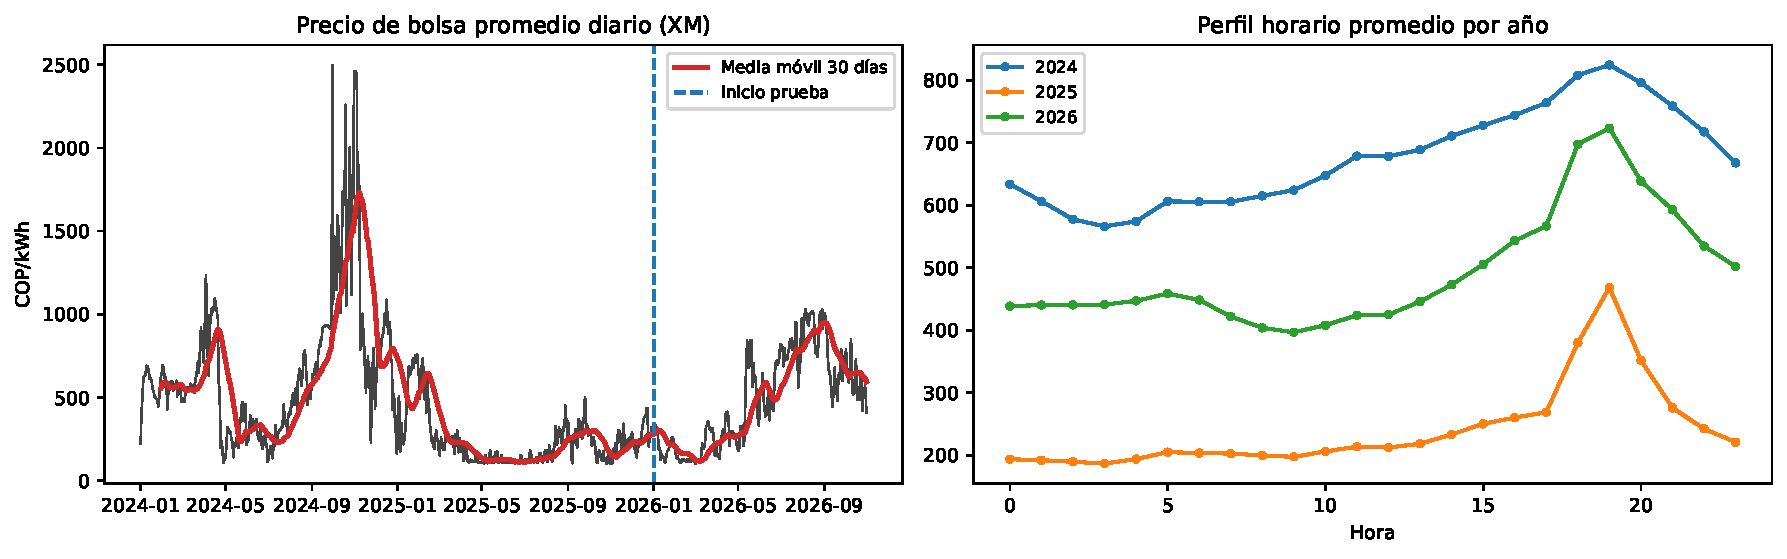
\includegraphics[width=0.88\linewidth]{precios_xm.pdf}
  \vspace{-6pt}
  \caption{Precio de bolsa diario con media móvil de 30 días (izq.) y perfil horario promedio por año (der.). Fuente: XM.}
  \label{fig:precios}
\end{figure}

% ─────────────────────────────────────────────────────────────────────────────
\section{Parte 1: MDP y aprendizaje por refuerzo}

\textbf{Formulación.} El estado es $s=(h,k,\ell)$:
\begin{itemize}
  \item $h$ es la hora;
  \item $k\in\{0,\dots,N\}$ es el nivel de carga, con $N$ = capacidad/potencia;
  \item $\ell$ es el nivel de precio: bajo, medio o alto según $p_t/\bar p_{d-1}$, con umbrales 0{,}85 y 1{,}15.
        Es una variable causal y relativa, para que la política no dependa del nivel absoluto de precios.
\end{itemize}
Las acciones son descargar, esperar o cargar. La recompensa es $-p_t e$ al cargar y $+p_t e \eta$ al descargar,
con $\eta = 0{,}9$ de ida y vuelta. Cada episodio es un día de 24 pasos que empieza con la batería vacía y
$\gamma = 1$. La recompensa acumulada es el ahorro frente a no tener batería.

\textbf{Métodos implementados por el equipo} (\texttt{src/politicas.py}):
\begin{enumerate}
  \item \textbf{Q-learning} (clase 5) con $\epsilon$-greedy, donde $\epsilon$ decrece de 1 a 0{,}05 en 200 épocas sobre
        los 731 días. La actualización es
        $Q(s,a)\leftarrow Q(s,a)+\alpha\,[\,r+\max_{a'}Q(s',a')-Q(s,a)\,]$.
        Dos ajustes salieron de los experimentos:
        (a) con $\alpha$ fijo la Q-table oscilaba por el ruido de los precios (solo capturaba entre 57\,\% y 67\,\% del oráculo),
        así que se usó $\alpha = 1/N(s,a)^{0.7}$;
        (b) al entrenar, la recompensa se divide por $\bar p_{d-1}$, porque los días de El Niño dominaban las actualizaciones.
  \item \textbf{Iteración de valor con modelo estimado} (clase 4). Se estiman $P(\ell'\mid h,\ell)$ y $E[p\mid h,\ell]$
        con los datos de entrenamiento y se resuelve Bellman de horizonte finito por inducción hacia atrás:
        $V_h(s)=\max_a\big[R(s,a)+\sum_{s'}T(s,a,s')\,V_{h+1}(s')\big]$, con $V_{24}=0$.
  \item \textbf{Líneas base:} \emph{horario fijo} (ingenua: carga en las $N$ horas más baratas del perfil promedio y
        descarga en las $N$ más caras) y \emph{aleatoria}.
  \item \textbf{Referencia:} un \emph{oráculo} que conoce los precios del día y se resuelve con programación dinámica.
        Es la cota superior.
\end{enumerate}

\textbf{Métrica:} ahorro en COP en el periodo de prueba y porcentaje del ahorro del oráculo.

\begin{table}[h]
  \centering\small
  \begin{tabular}{lcccc}
    \toprule
    Batería (prueba 2026) & Q-learning (5 semillas) & Iter.\ de valor & Horario fijo & Aleatoria \\
    \midrule
    10 kWh / 2,5 kW  & \textbf{77,7 $\pm$ 1,7\,\%} & 75,8\,\% & 72,3\,\% & $-$146,6\,\% \\
    10 kWh / 5 kW    & \textbf{76,8 $\pm$ 3,3\,\%} & 76,6\,\% & 70,6\,\% & $-$126,1\,\% \\
    10 kWh / 1,25 kW & \textbf{81,3 $\pm$ 2,1\,\%} & 80,5\,\% & 73,0\,\% & $-$148,5\,\% \\
    \bottomrule
  \end{tabular}
  \caption{Porcentaje del ahorro del oráculo capturado en el periodo de prueba (datos no vistos).}
  \label{tab:resultados}
\end{table}

En la configuración por defecto, el oráculo ahorra 649.756~COP en 304 días, Q-learning 484.607~COP (semilla 42)
y el horario fijo 469.599~COP (Fig.~\ref{fig:ahorro}). Las dos políticas aprendidas superan a la ingenua en las tres
configuraciones y capturan cerca de $\frac34$ de la cota superior.

La política aprendida carga de madrugada (0--3~h) y descarga entre las 18 y las 21~h (Fig.~\ref{fig:patron}).
A diferencia del horario fijo, \textbf{reacciona al precio del día}: no carga de madrugada si el nivel de precio es alto
y aprovecha un segundo ciclo parcial por la tarde (descarga a las 15--16~h y recarga a las 17~h, antes del pico).
Por eso hace más ciclos equivalentes (346 frente a 304). La Fig.~\ref{fig:semana} muestra estas decisiones en una semana de prueba.

\begin{figure}[h]
  \centering
  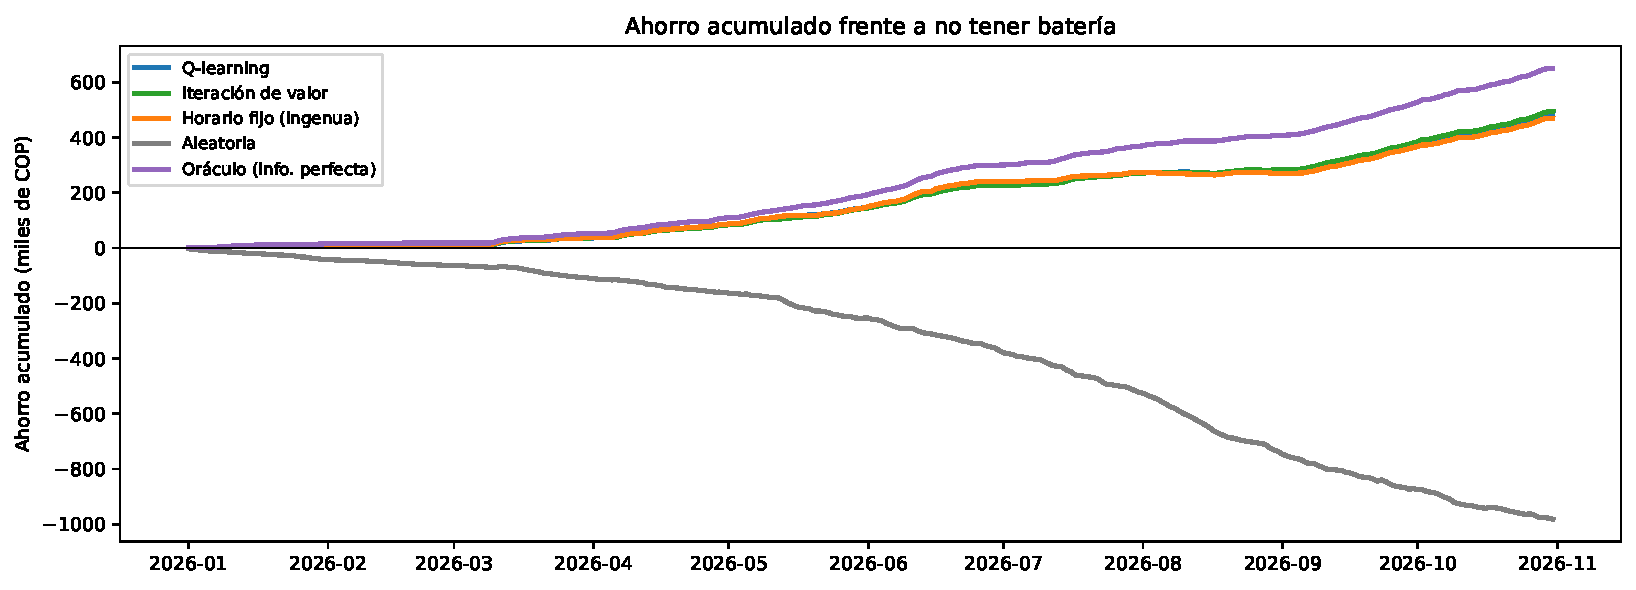
\includegraphics[width=0.76\linewidth]{ahorro_acumulado.pdf}
  \vspace{-6pt}
  \caption{Ahorro acumulado en 2026 frente a no tener batería (10 kWh, 2,5 kW, $\eta=0{,}9$).}
  \label{fig:ahorro}
\end{figure}

\begin{figure}[h]
  \centering
  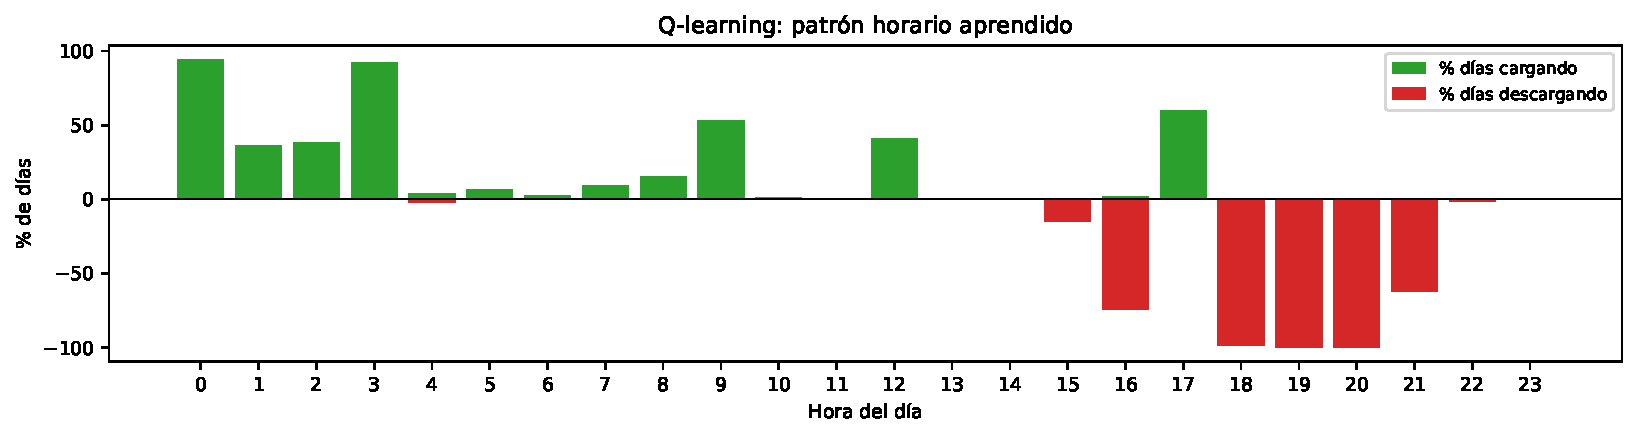
\includegraphics[width=0.76\linewidth]{patron_horario.pdf}
  \vspace{-6pt}
  \caption{Porcentaje de días de 2026 en que Q-learning carga (verde) o descarga (rojo) en cada hora.}
  \label{fig:patron}
\end{figure}

\begin{figure}[h]
  \centering
  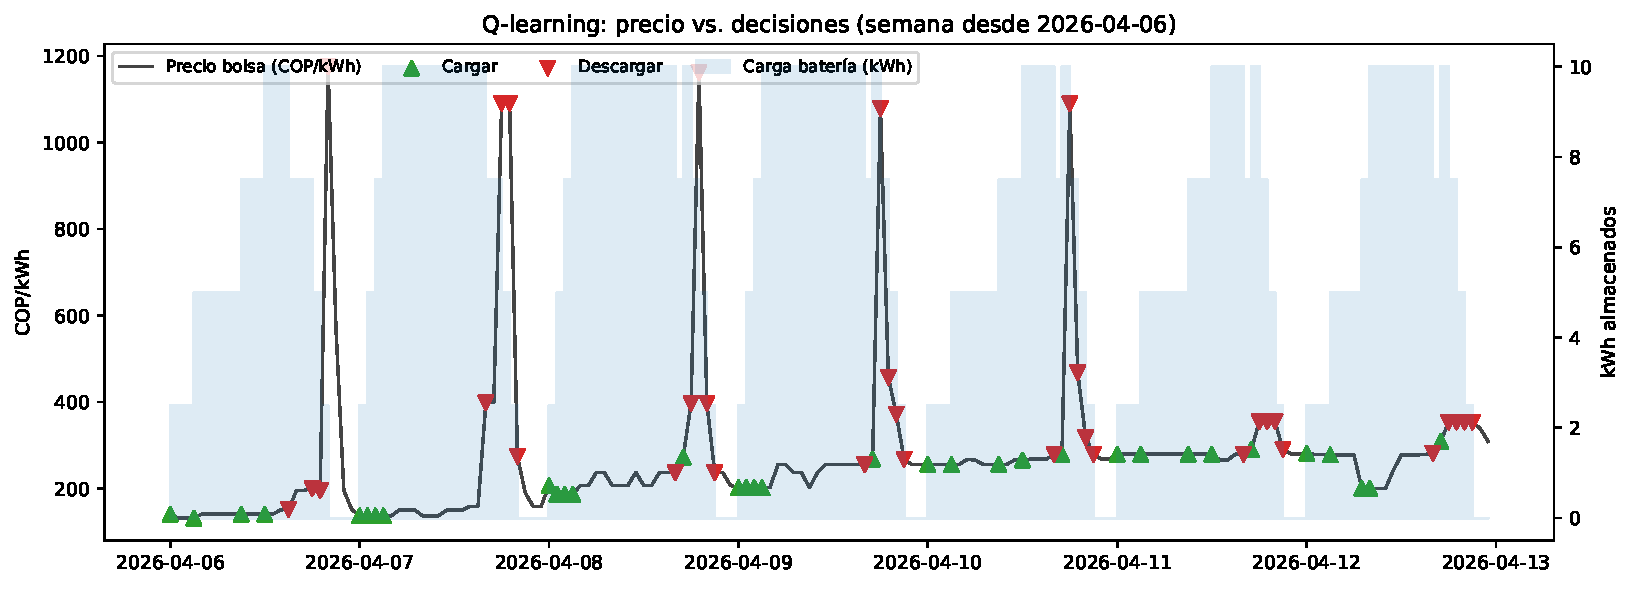
\includegraphics[width=0.76\linewidth]{decisiones_semana.pdf}
  \vspace{-6pt}
  \caption{Precio de bolsa y decisiones de Q-learning durante una semana de prueba. El área azul es la energía almacenada.}
  \label{fig:semana}
\end{figure}

% ─────────────────────────────────────────────────────────────────────────────
\section{Parte 2: Agente LLM con RAG}

\begin{itemize}
  \item \textbf{Loop agéntico manual} (clase 11) sobre un endpoint compatible con OpenAI (NVIDIA NIM,
        \texttt{nemotron-3.5-super-vl-120b-a12b}), con $T_{\max}=6$ iteraciones. Los errores de las herramientas
        (fechas fuera de rango, política inexistente, JSON inválido) se devuelven al modelo como observación.
  \item \textbf{RAG:} chunking semántico (hasta 900 caracteres), embeddings \texttt{nemotron-3-embed-1b} normalizados y
        FAISS \texttt{IndexFlatIP} (coseno) con umbral 0{,}25. Las preguntas fuera de dominio no recuperan fragmentos.
  \item \textbf{Herramientas:}
        \texttt{consultar\_precios} (datos de XM),
        \texttt{simular} (ejecuta el MDP de la Parte~1 y compara todas las políticas) y
        \texttt{buscar\_documentos} (RAG). El LLM no calcula nada: recibe el JSON de la simulación como observación
        y redacta con esas cifras. El system prompt exige usar herramientas para cualquier cifra y citar
        \texttt{[Resolución\,\dots]}, \texttt{[XM]} o \texttt{[Simulación MDP]}.
\end{itemize}

\textbf{Evaluación con 13 preguntas fijas} (datos, simulación, explicación, RAG, multi-herramienta, caso límite y fuera de
alcance):
\begin{itemize}
  \item Herramienta correcta: \textbf{12/13 (92\,\%)}. Cita correcta: \textbf{13/13 (100\,\%)}. En promedio usó 1,8 iteraciones.
  \item Todas las cifras reportadas coinciden con los valores calculados directamente de los datos.
  \item El único fallo es el caso límite ``precio en 2030'': el agente respondió bien que no hay datos, pero sin llamar
        la herramienta, porque el system prompt ya le informa el rango.
  \item En la pregunta sobre arbitraje, el agente distinguió lo que afirma el fragmento recuperado (la política del
        MinEnergía faculta a la CREG para reglar el arbitraje) de lo que no confirma.
\end{itemize}

% ─────────────────────────────────────────────────────────────────────────────
\section{Dashboard}

Aplicación Gradio (\texttt{python app.py}) con tres pestañas:
\begin{itemize}
  \item \textbf{Simulación:} el usuario elige la política, el rango de fechas, la capacidad, la potencia y la eficiencia.
        Muestra una tabla comparativa y las Figs.~\ref{fig:ahorro}--\ref{fig:semana}.
  \item \textbf{Datos XM:} las series de la Fig.~\ref{fig:precios}.
  \item \textbf{Asistente:} chat con traza visible de las herramientas, sus argumentos y las fuentes, con enlace a la CREG.
\end{itemize}

% ─────────────────────────────────────────────────────────────────────────────
\section{Limitaciones y trabajo futuro}

\begin{itemize}
  \item \textbf{Modelo simplificado:} 3 niveles de precio, pasos de 1 hora, sin degradación ni autodescarga, y la batería
        empieza vacía cada día. Un usuario regulado no paga el precio de bolsa directamente, así que el ahorro es un
        arbitraje teórico.
  \item \textbf{Información:} el precio de bolsa se publica después de la hora. En el MDP se supone observable en la hora
        de decisión, aunque el nivel de precio solo usa el día anterior como referencia.
  \item \textbf{Margen sobre el horario fijo:} es moderado (+3 a +8 puntos) porque el perfil horario colombiano es muy regular.
        Variables como el nivel de los embalses o la demanda, también disponibles en XM, podrían mejorarlo.
  \item \textbf{Radiación solar:} no se incorporó la del IDEAM, que permitiría el escenario de batería con paneles.
  \item \textbf{Agente:} el LLM no es determinista, la verificación de citas es sintáctica y el corpus solo tiene 4 normas.
  \item \textbf{Uso:} es una herramienta académica y no constituye asesoría financiera, legal ni de seguridad.
\end{itemize}

\end{document}
